\section{Ergebnis}
Alle bereits beschriebenen Bibliotheken, Pakete und Methoden fügen sich zu einer finalen Applikation zusammen.
Diese ermöglicht es dem Nutzer Zeiten zu erfassen und benachrichtigt ihn bei bestimmten Ereignissen.

Die Screenshots der Anwendung in \autoref{fig:screenshots} zeigen den Fortschritt der Applikation.
Im Vergleich zu den Mockups wirkt die Anwendung deutlich ansprechender.
In bestimmten Details sind auch weitere Optimierungen erkennbar.

Insgesamt kann die Anwendung als funktionsfähig bezeichnet werden,
wenn es auch an der ein oder anderen Stelle Raum für Verbesserungen gibt.

\begin{figure}[h]
    \centering
    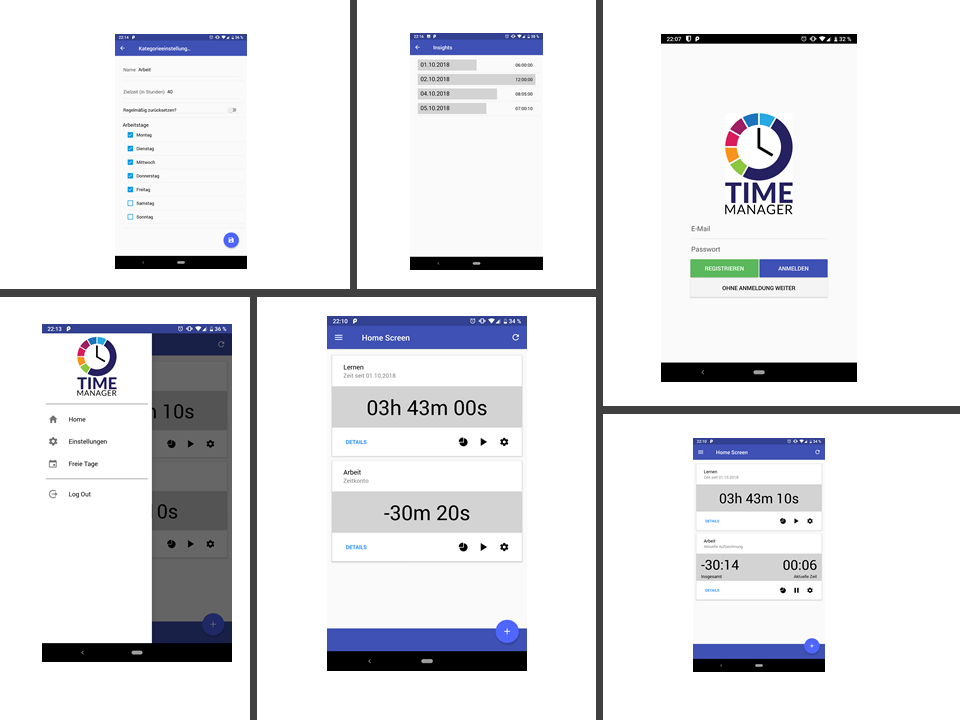
\includegraphics[width=\textwidth]{Final_App}
    \caption{Screenshots der Applikation}
    \label{fig:screenshots}
\end{figure}